% 20120531-093353-093653
% A-0.5/W20.7

\section{A-0.5/W20.7 - 130 krpm}
\label{sec:awp-exp-details-A-0.5/W20.7}

This test has been performed on May 31\th{} 2012, between 09:33:53 and
09:36:53.

\begin{figure}[htbp]
  \centering
  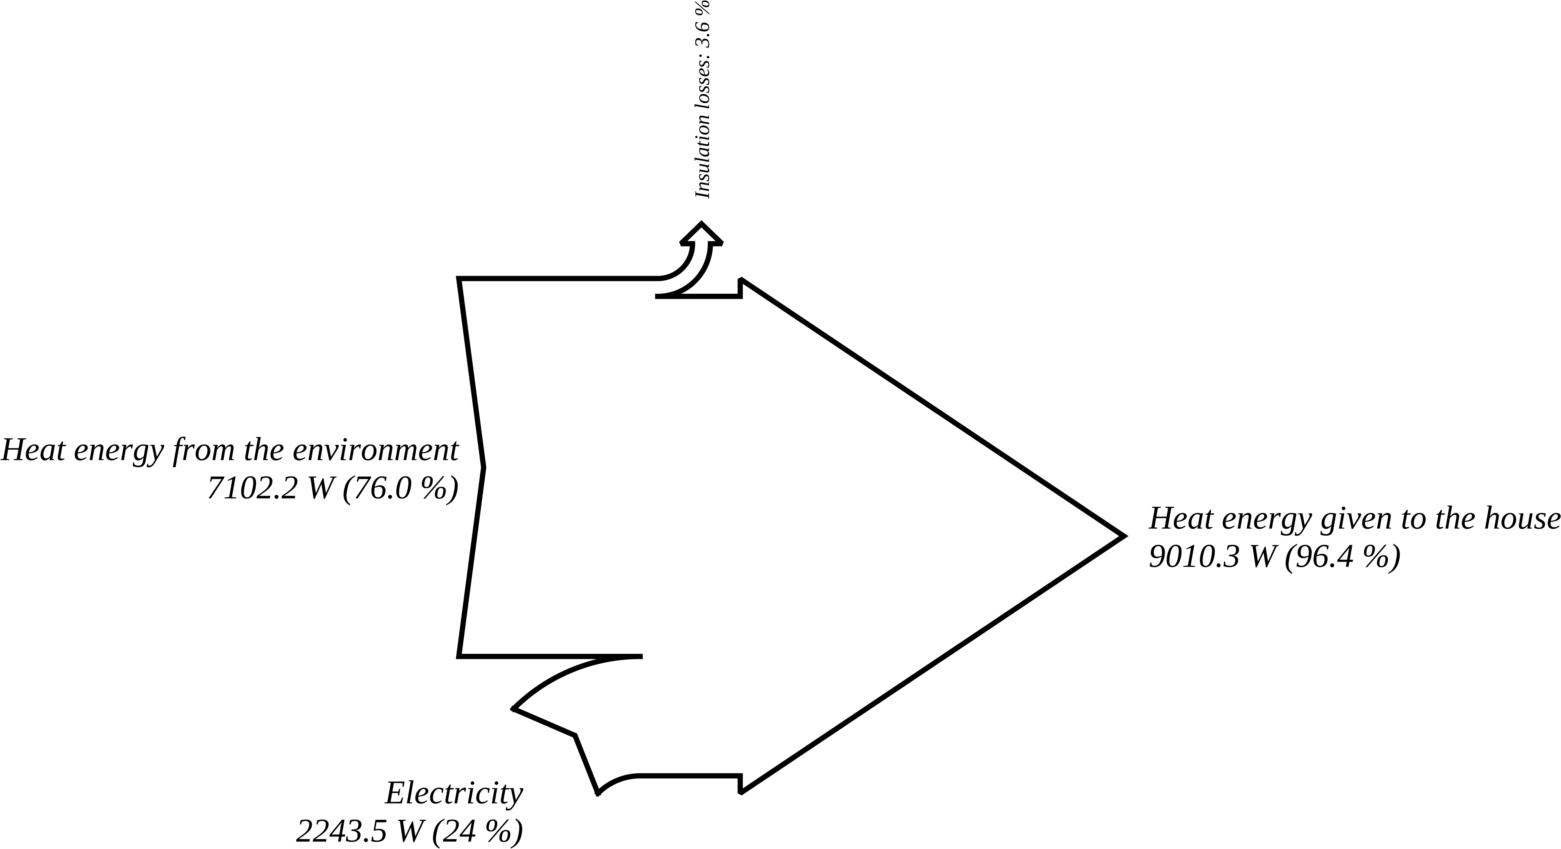
\includegraphics[width=0.7\textwidth]{awp-energy-sankey-awp-20120531-093353-093653}
  \caption{A-0.5/W20.7 -- Sankey diagram for heat pump energy balance (internal frontier)}
  \label{fig:awp-A-0.5/W20.7-sankey-energy}
\end{figure}


\begin{figure}[htbp]
  \centering
  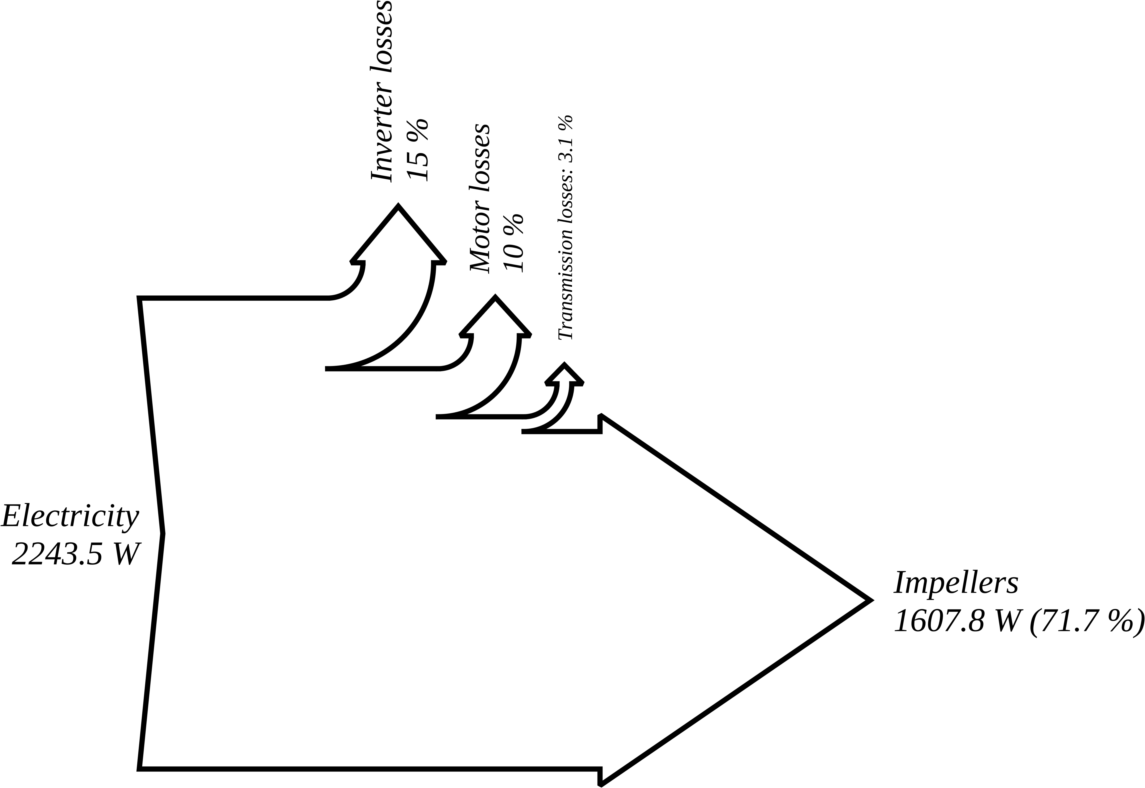
\includegraphics[width=0.7\textwidth]{awp-energy-sankey-cp-20120531-093353-093653}
  \caption{A-0.5/W20.7 -- Sankey diagram for the compressor unit energy balance}
  \label{fig:awp-A-0.5/W20.7-sankey-cp}
\end{figure}

\begin{figure}[htbp]
  \centering
  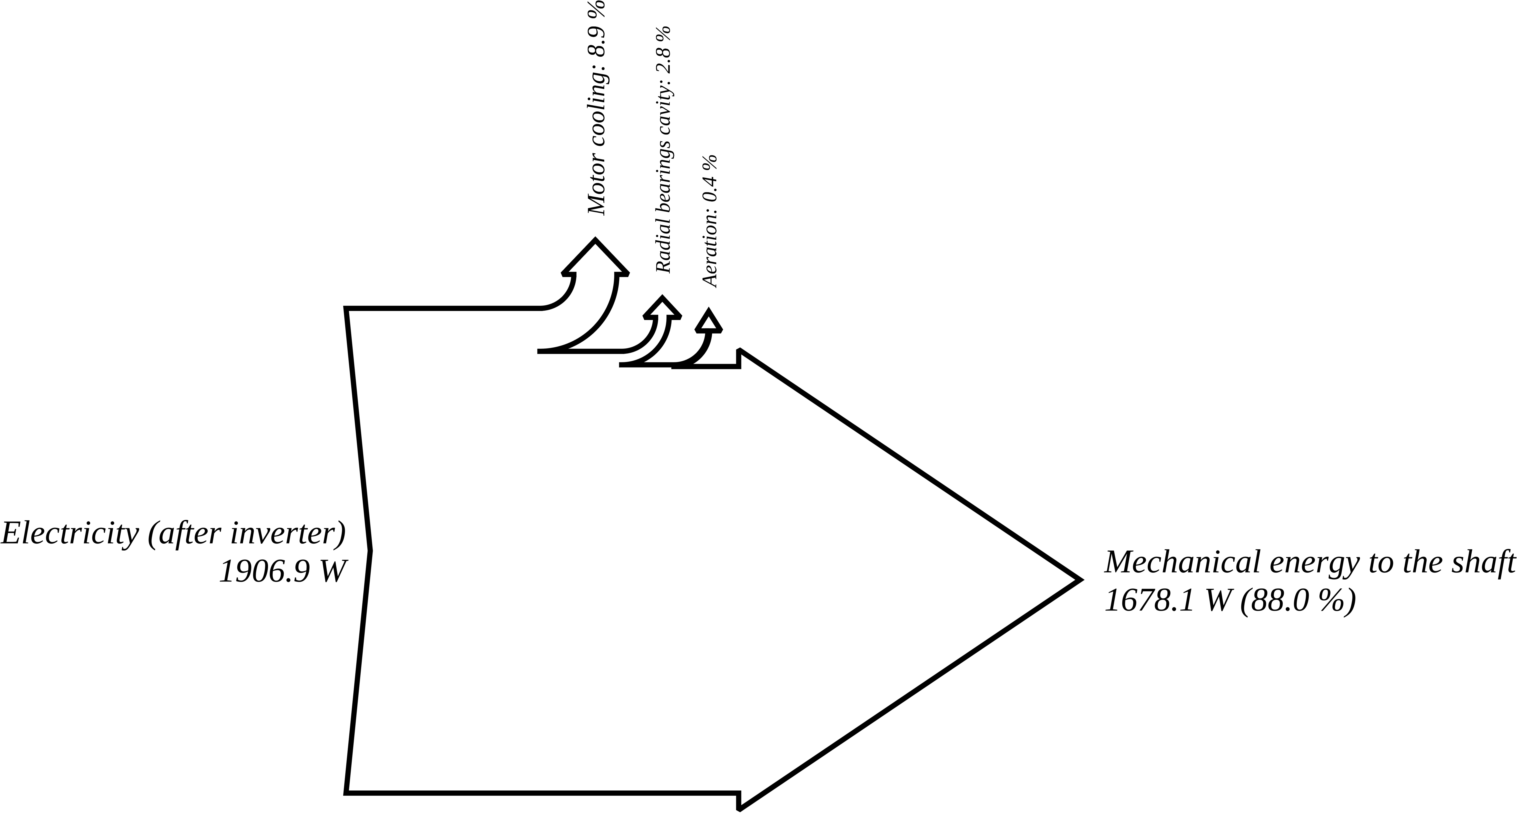
\includegraphics[width=0.7\textwidth]{awp-energy-sankey-motor-20120531-093353-093653}
  \caption{A-0.5/W20.7 -- Sankey diagram for the motor energy balance}
  \label{fig:awp-A-0.5/W20.7-sankey-motor}
\end{figure}

\begin{table}[htbp]
    \footnotesize
    \begin{center}
    \begin{tabular}{llllll}
\toprule
Name & Value / \% & Name & Value / \% & Name & Value / - \\
\midrule
$\eta_{heatpump}$ & $ \num{26.6} \pm \num{0.8} $ & $\eta_{mot}$ & $ \num{87.9} \pm \num{0.2} $ & $\epsilon_h$ & $ \num{4.02} \pm \num{0.06} $\\
$\eta_{cp1}$ & $ \num{78} \pm \num{21} $ & $\eta_{cp2}$ &$ \num{53} \pm \num{34} $ & $\pi_1$ & $ \num{1.847} \pm \num{0.001} $\\
$\eta_{cp1,\,imp}$ & $ \num{76} \pm \num{23} $ & $\eta_{cp2,\,imp}$ & $ \num{66} \pm \num{34} $ & $\pi_2$ & $ \num{1.6787} \pm \num{7e-04} $\\
$\eta_{cd}$ & $ \num{89} \pm \num{3} $ & $\eta_{ev}$ & $ \num{29} \pm \num{29} $ & $\pi_{1,\,theory}$ & $ \num{1.9} \pm \num{0.2} $\\
$\eta_{trans}$ & $ \num{95.81} \pm \num{0.03} $ & $\eta_{sc}$ & $ \num{3} \pm \num{3} $ & $\pi_{2,\,theory}$ & N/A\\
$\eta_{s,\,cp1}$ & $ \num{93} \pm \num{7} $ & $\eta_{s,\,cp2}$ & $ \num{89} \pm \num{11} $ & $\eta_{mot}$ & $\underline{88.00}$ \%\\
$\eta_{s,\,cp1,\,ext}$ & $99.20$ & $\eta_{s,\,cp2,\,ext}$ & $ \num{39} \pm \num{39} $ & $\eta_{radial}$ & $ \num{98.45} \pm \num{0.03} $ \%\\
$\eta_{s,\,cp1,\,theory}$ & $ \num{79} \pm \num{2} $ & $\eta_{s,\,cp2,\,theory}$ & N/A & $\eta_{axial}$ & $ \num{97.31} \pm \num{0.03} $ \%\\
\bottomrule
\end{tabular}

  \end{center}
  \caption{A-0.5/W20.7 -- Performance indicators}
\end{table}

\begin{table}[htbp]
  \footnotesize
  \begin{center}
    \begin{tabular}{cccccc}
\toprule
Component & Location & P / \si{\bar} & T / \si{\degreeCelsius} & h / \si{\kilo\joule\per\kilo\gram} & s / \si{\kilo\joule\per\kilo\gram\per\kelvin}\\
\midrule
\multirow{2}{*}{1} & inlet & $ \num{2.017} \pm \num{0.001} $ & $ \num{3} \pm \num{13} $ & $ \num{403.92} \pm \num{0.02} $ & $ \num{1.77} \pm \num{0.04} $\\
& outlet & $ \num{3.725} \pm \num{0.001} $ & $ \num{28} \pm \num{2} $ & $ \num{421.988} \pm \num{0.002} $ & $ \num{1.791} \pm \num{0.006} $\\
\midrule
\multirow{2}{*}{2} & inlet & $\pmb{ \num{3.725} \pm \num{0.001} }$ & $\pmb{ \num{11.125} \pm \num{0.006} }$ & $ \num{406.504319} \pm \num{6e-06} $ & $ \num{1.73763} \pm \num{6e-05} $\\
& outlet & $\pmb{ \num{6.254} \pm \num{0.001} }$ & $\pmb{ \num{32.140} \pm \num{0.006} }$ & $ \num{420.500606} \pm \num{6e-06} $ & $ \num{1.74764} \pm \num{5e-05} $\\
\midrule
\multirow{2}{*}{3} & inlet & $\pmb{ \num{5.936} \pm \num{0.001} }$ & $\pmb{ \num{31.015} \pm \num{0.005} }$ & $ \num{420.101398} \pm \num{5e-06} $ & $ \num{1.75005} \pm \num{4e-05} $\\
& outlet & $\pmb{ \num{5.841} \pm \num{0.001} }$ & $\pmb{ \num{17.638} \pm \num{0.005} }$ & $ \num{224.162130} \pm \num{5e-06} $ & $ \num{1.08488} \pm \num{2e-05} $\\
\midrule
\multirow{2}{*}{4} & inlet & $ \num{2.092} \pm \num{0.001} $ & $ \num{-8.9} \pm \num{0.6} $ & $ \num{219.9442} \pm \num{6e-04} $ & $ \num{1.076} \pm \num{0.003} $\\
& outlet & $\pmb{ \num{2.079} \pm \num{0.001} }$ & $\pmb{ \num{-1.960} \pm \num{0.005} }$ & $ \num{399.313756} \pm \num{5e-06} $ & $ \num{1.75553} \pm \num{8e-05} $\\
\midrule
\multirow{2}{*}{5} & inlet & $ \num{5.841} \pm \num{0.001} $ & $ \num{17.64} \pm \num{0.04} $ & $ \num{224.16213} \pm \num{4e-05} $ & $ \num{1.0849} \pm \num{2e-04} $\\
& outlet & $ \num{3.725} \pm \num{0.001} $ & $ \num{6.8} \pm \num{0.5} $ & $ \num{224.1621} \pm \num{4e-04} $ & $ \num{1.086} \pm \num{0.002} $\\
\midrule
\multirow{2}{*}{6} & inlet & $ \num{3.725} \pm \num{0.001} $ & $ \num{6.3} \pm \num{0.6} $ & $ \num{208.4875} \pm \num{5e-04} $ & $ \num{1.030} \pm \num{0.003} $\\
& outlet & $ \num{2.343} \pm \num{0.001} $ & $ \num{-6.0} \pm \num{0.6} $ & $ \num{208.4875} \pm \num{6e-04} $ & $ \num{1.032} \pm \num{0.003} $\\
\midrule
\multirow{2}{*}{7} & inlet & $ \num{2.343} \pm \num{0.001} $ & $ \num{-6.0} \pm \num{0.6} $ & $ \num{224.1621} \pm \num{6e-04} $ & $ \num{1.091} \pm \num{0.002} $\\
& outlet & $ \num{2.343} \pm \num{0.001} $ & $ \num{36} \pm \num{8} $ & $ \num{432.166} \pm \num{0.008} $ & $ \num{1.86} \pm \num{0.02} $\\
\midrule
\multirow{2}{*}{8} & inlet & $\pmb{ \num{3.725} \pm \num{0.001} }$ & $\pmb{ \num{6.836} \pm \num{0.006} }$ & $ \num{402.537415} \pm \num{6e-06} $ & $ \num{1.7236} \pm \num{4e-04} $\\
& outlet & $ \num{3.73} \pm \num{0.05} $ & $ \num{6.8} \pm \num{0.5} $ & $ \num{209.2490} \pm \num{4e-04} $ & $ \num{1.033} \pm \num{0.002} $\\
\midrule
\multirow{2}{*}{9} & inlet & $\pmb{ \num{2.343} \pm \num{0.001} }$ & $\pmb{ \num{-5.994} \pm \num{0.005} }$ & $ \num{219.944179} \pm \num{5e-06} $ & $ \num{1.07515} \pm \num{7e-05} $\\
& outlet & $ \num{2.092} \pm \num{0.001} $ & $ \num{-8.9} \pm \num{0.6} $ & $ \num{219.9442} \pm \num{6e-04} $ & $ \num{1.076} \pm \num{0.003} $\\
\midrule
\multirow{2}{*}{10} & inlet & $ \num{6.254} \pm \num{0.001} $ & $ \num{32} \pm \num{2} $ & $ \num{420.501} \pm \num{0.001} $ & $ \num{1.748} \pm \num{0.005} $\\
& outlet & $ \num{3.725} \pm \num{0.001} $ & $ \num{46} \pm \num{21} $ & $ \num{438.91} \pm \num{0.03} $ & $ \num{1.85} \pm \num{0.06} $\\
\midrule
\multirow{2}{*}{11} & inlet & $ \num{2.017} \pm \num{0.001} $ & $ \num{125} \pm \num{47} $ & $ \num{516.61} \pm \num{0.05} $ & $ \num{2.1} \pm \num{0.1} $\\
& outlet & $ \num{2.017} \pm \num{0.001} $ & $ \num{123} \pm \num{57} $ & $ \num{514.63} \pm \num{0.06} $ & $ \num{2.1} \pm \num{0.1} $\\
\midrule
\multirow{2}{*}{12} & inlet & $ \num{2.143} \pm \num{0.001} $ & $ \num{13} \pm \num{21} $ & $ \num{411.80} \pm \num{0.03} $ & $ \num{1.80} \pm \num{0.06} $\\
& outlet & $ \num{2.143} \pm \num{0.001} $ & $ \num{86} \pm \num{43} $ & $ \num{477.63} \pm \num{0.05} $ & $ \num{2.0} \pm \num{0.1} $\\
\midrule
\multirow{2}{*}{13} & inlet & $ \num{2.143} \pm \num{0.001} $ & $ \num{6} \pm \num{3} $ & $ \num{406.191} \pm \num{0.002} $ & $ \num{1.778} \pm \num{0.008} $\\
& outlet & $ \num{2.143} \pm \num{0.001} $ & $ \num{14} \pm \num{22} $ & $ \num{412.95} \pm \num{0.03} $ & $ \num{1.80} \pm \num{0.07} $\\
\midrule
\multirow{2}{*}{15} & inlet & & $\pmb{ \num{14.453} \pm \num{0.005} }$ & \multicolumn{2}{l}{Cp = $ \num{4188.728} \pm \num{0.006} $ \si{\joule\per\kilo\gram\per\kelvin}}\\
& outlet & & $\pmb{ \num{20.716} \pm \num{0.005} }$ & \multicolumn{2}{l}{Cp = $ \num{4183.264} \pm \num{0.004} $ \si{\joule\per\kilo\gram\per\kelvin}}\\
\midrule
\multirow{2}{*}{16} & inlet & & $\pmb{ \num{-0.495} \pm \num{0.005} }$ & & \\
& outlet & & $\pmb{ \num{-4.827} \pm \num{0.005} }$ & & \\
\midrule
\multirow{2}{*}{18} & inlet & $ \num{2.079} \pm \num{0.001} $ & $ \num{-2} \pm \num{2} $ & $ \num{399.314} \pm \num{0.002} $ & $ \num{1.756} \pm \num{0.008} $\\
& outlet & $\pmb{ \num{2.017} \pm \num{0.001} }$ & $\pmb{ \num{-1.311} \pm \num{0.009} }$ & $ \num{400.036209} \pm \num{9e-06} $ & $ \num{1.7605} \pm \num{1e-04} $\\
\midrule
\multirow{2}{*}{19} & inlet & $ \num{3.725} \pm \num{0.001} $ & $ \num{6.8} \pm \num{0.5} $ & $ \num{209.2490} \pm \num{4e-04} $ & $ \num{1.033} \pm \num{0.002} $\\
& outlet & $ \num{3.725} \pm \num{0.001} $ & $ \num{6.3} \pm \num{0.6} $ & $ \num{208.4875} \pm \num{5e-04} $ & $ \num{1.030} \pm \num{0.003} $\\
\midrule
\multirow{2}{*}{20} & inlet & $ \num{6.254} \pm \num{0.001} $ & $ \num{32} \pm \num{2} $ & $ \num{420.501} \pm \num{0.001} $ & $ \num{1.748} \pm \num{0.005} $\\
& outlet & $ \num{5.936} \pm \num{0.001} $ & $ \num{31} \pm \num{2} $ & $ \num{420.101} \pm \num{0.001} $ & $ \num{1.750} \pm \num{0.005} $\\
\midrule
\multirow{2}{*}{21} & inlet & $ \num{2.143} \pm \num{0.001} $ & $ \num{6} \pm \num{3} $ & $ \num{406.191} \pm \num{0.002} $ & $ \num{1.778} \pm \num{0.008} $\\
& outlet & $\pmb{ \num{2.173} \pm \num{0.001} }$ & $\pmb{ \num{6.271} \pm \num{0.006} }$ & $ \num{406.116899} \pm \num{6e-06} $ & $ \num{1.77684} \pm \num{8e-05} $\\
\midrule
\multirow{2}{*}{22} & inlet & $ \num{2.017} \pm \num{0.001} $ & $ \num{0} \pm \num{10} $ & $ \num{401.19} \pm \num{0.02} $ & $ \num{1.76} \pm \num{0.03} $\\
& outlet & $\pmb{ \num{2.017} \pm \num{0.001} }$ & $\pmb{ \num{0.041} \pm \num{0.006} }$ & $ \num{401.187210} \pm \num{6e-06} $ & $ \num{1.76473} \pm \num{9e-05} $\\
\midrule
\multirow{2}{*}{23} & inlet & $ \num{2.017} \pm \num{0.001} $ & $ \num{123} \pm \num{57} $ & $ \num{514.63} \pm \num{0.06} $ & $ \num{2.1} \pm \num{0.1} $\\
& outlet & $ \num{2.017} \pm \num{0.001} $ & $ \num{124} \pm \num{64} $ & $ \num{515.10} \pm \num{0.07} $ & $ \num{2.1} \pm \num{0.2} $\\
\midrule
\multirow{2}{*}{24} & inlet & $ \num{2.017} \pm \num{0.001} $ & $ \num{85} \pm \num{43} $ & $ \num{477.63} \pm \num{0.05} $ & $ \num{2.0} \pm \num{0.1} $\\
& outlet & $ \num{2.017} \pm \num{0.001} $ & $ \num{125} \pm \num{47} $ & $ \num{516.61} \pm \num{0.05} $ & $ \num{2.1} \pm \num{0.1} $\\
\midrule
\multirow{2}{*}{25} & inlet & $ \num{3.725} \pm \num{0.001} $ & $ \num{28} \pm \num{13} $ & $ \num{425.58} \pm \num{0.02} $ & $ \num{1.80} \pm \num{0.04} $\\
& outlet & $\pmb{ \num{3.725} \pm \num{0.001} }$ & $\pmb{ \num{31.979} \pm \num{0.006} }$ & $ \num{425.577035} \pm \num{6e-06} $ & $ \num{1.80238} \pm \num{6e-05} $\\
\midrule
\multirow{2}{*}{26} & inlet & $ \num{6.254} \pm \num{0.001} $ & $ \num{32} \pm \num{2} $ & $ \num{420.501} \pm \num{0.001} $ & $ \num{1.748} \pm \num{0.005} $\\
& outlet & $\pmb{ \num{2.143} \pm \num{0.001} }$ & $\pmb{ \num{6.271} \pm \num{0.006} }$ & $ \num{406.191435} \pm \num{6e-06} $ & $ \num{1.77819} \pm \num{8e-05} $\\
\midrule
\multirow{2}{*}{27} & inlet & $ \num{3.725} \pm \num{0.001} $ & $ \num{28} \pm \num{2} $ & $ \num{421.988} \pm \num{0.001} $ & $ \num{1.791} \pm \num{0.005} $\\
& outlet & $ \num{3.725} \pm \num{0.001} $ & $ \num{28} \pm \num{2} $ & $ \num{421.988} \pm \num{0.001} $ & $ \num{1.791} \pm \num{0.005} $\\
\midrule
\multirow{2}{*}{28} & inlet & $ \num{3.725} \pm \num{0.001} $ & $ \num{6.8} \pm \num{0.5} $ & $ \num{402.5374} \pm \num{4e-04} $ & $ \num{1.724} \pm \num{0.001} $\\
& outlet & $ \num{3.725} \pm \num{0.001} $ & $ \num{11} \pm \num{2} $ & $ \num{406.504} \pm \num{0.002} $ & $ \num{1.738} \pm \num{0.006} $\\
\midrule
\multirow{2}{*}{29} & inlet & $ \num{2.017} \pm \num{0.001} $ & $ \num{1} \pm \num{11} $ & $ \num{401.80} \pm \num{0.02} $ & $ \num{1.77} \pm \num{0.04} $\\
& outlet & $ \num{2.017} \pm \num{0.001} $ & $ \num{1} \pm \num{11} $ & $ \num{401.80} \pm \num{0.02} $ & $ \num{1.77} \pm \num{0.04} $\\
\bottomrule
\end{tabular}

  \end{center}
  \caption{A-0.5/W20.7 -- Thermodynamic points of the heat pump cycle}
  \label{tab:A-0.5/W20.7-PThs}
\end{table}


\begin{table}[htbp]
    \footnotesize
    \begin{center}
    \begin{tabular}{llllll}
\toprule
Name & Value / \si{\gram\per\second} & Name & Value / \si{\gram\per\second} & Name & Value / \si{\gram\per\second} \\
\midrule
$\dot{M}_{1 \rightarrow 25}$ & $ \num{35.4} \pm \num{0.8} $ & $\dot{M}_{2 \rightarrow 10}$ & $\underline{9.52}$ & $\dot{M}_{2 \rightarrow 20}$ & $ \num{46.0} \pm \num{0.8} $ \\
$\dot{M}_{2 \rightarrow 26}$ & $\pmb{ \num{1.20} \pm \num{1.20} }$ & $\dot{M}_{3 \rightarrow 5}$ & $ \num{44.2} \pm \num{0.8} $ & $\dot{M}_{3 \rightarrow 7}$ & $\pmb{ \num{1.75} \pm \num{1.75} }$ \\
$\dot{M}_{4 \rightarrow 18}$ & $ \num{34.2} \pm \num{0.8} $ & $\dot{M}_{5 \rightarrow 8}$ & $ \num{44.2} \pm \num{0.8} $ & $\dot{M}_{6 \rightarrow 9}$ & $ \num{32.4} \pm \num{0.8} $ \\
$\dot{M}_{7 \rightarrow 9}$ & $ \num{1.75} \pm \num{1.75} $ & $\dot{M}_{8 \rightarrow 19}$ & $ \num{32.4} \pm \num{0.8} $ & $\dot{M}_{8 \rightarrow 28}$ & $ \num{45} \pm \num{2} $ \\
$\dot{M}_{9 \rightarrow 4}$ & $ \num{34.2} \pm \num{0.8} $ & $\dot{M}_{10 \rightarrow 25}$ & $9.52$ & $\dot{M}_{11 \rightarrow 22}$ & $ \num{1.19} \pm \num{1.19} $ \\
$\dot{M}_{11 \rightarrow 23}$ & $ \num{0.0148} \pm \num{1e-02} $ & $\dot{M}_{12 \rightarrow 24}$ & $ \num{1.20} \pm \num{1.20} $ & $\dot{M}_{13 \rightarrow 12}$ & $ \num{1.00} \pm \num{1.00} $ \\
$\dot{M}_{17 \rightarrow 15}$ & $\pmb{ \num{366} \pm \num{4} }$ & $\dot{M}_{18 \rightarrow 22}$ & $ \num{34.2} \pm \num{0.8} $ & $\dot{M}_{19 \rightarrow 6}$ & $ \num{32.4} \pm \num{0.8} $ \\
$\dot{M}_{20 \rightarrow 3}$ & $ \num{46.0} \pm \num{0.8} $ & $\dot{M}_{21 \rightarrow 12}$ & $ \num{0.20} \pm \num{0.20} $ & $\dot{M}_{22 \rightarrow 29}$ & $ \num{35.4} \pm \num{0.8} $ \\
$\dot{M}_{23 \rightarrow 29}$ & $ \num{0.0148} \pm \num{1e-02} $ & $\dot{M}_{24 \rightarrow 11}$ & $ \num{1.20} \pm \num{1.20} $ & $\dot{M}_{25 \rightarrow 8}$ & $ \num{33.3} \pm \num{0.6} $ \\
$\dot{M}_{25 \rightarrow 27}$ & $ \num{11.6} \pm \num{0.2} $ & $\dot{M}_{26 \rightarrow 13}$ & $ \num{1.00} \pm \num{1.00} $ & $\dot{M}_{26 \rightarrow 21}$ & $ \num{0.20} \pm \num{0.20} $ \\
$\dot{M}_{27 \rightarrow 28}$ & $ \num{11.6} \pm \num{0.2} $ & $\dot{M}_{28 \rightarrow 2}$ & $ \num{57} \pm \num{2} $ & $\dot{M}_{29 \rightarrow 1}$ & $ \num{35.4} \pm \num{0.8} $ \\
$\dot{M}_{cp_1}$ & $ \num{35.4} \pm \num{0.8} $ & $\dot{M}_{cp_2}$ & $ \num{56.7} \pm \num{0.8} $ \\
\bottomrule
\end{tabular}

  \end{center}
  \caption{A-0.5/W20.7 -- Mass flow rates between the components}
  \label{tab:awp-A-0.5/W20.7-mf}
\end{table}

\begin{table}[htbp]
    \footnotesize
    \begin{center}
    \begin{tabular}{llll}
\toprule
Name & Value / $W$ & Name & Value / $W$ \\
\midrule
$\dot{E}_{1 \rightarrow 2}$ & $ \num{969} \pm \num{605} $ & $\dot{E}_{11 \rightarrow 1}$ & $ \num{1607.8} \pm \num{0.3} $ \\
$\dot{E}_{12 \rightarrow 11}$ & $ \num{1652.2} \pm \num{0.3} $ & $\dot{E}_{13 \rightarrow 12}$ & $ \num{1678.1} \pm \num{0.3} $ \\
$\dot{E}_{14 \rightarrow 13}$ & $ \num{1906.9} \pm \num{0.3} $ & $\dot{E}_{el \rightarrow 14}$ & $\pmb{ \num{2243.5} \pm \num{0.4} }$ \\
$\dot{Y}_{1 \rightarrow 2}$ & $ \num{0.003} \pm \num{0.003} $ & $\dot{Y}_{2 \rightarrow 10}$ & $ \num{175} \pm \num{175} $ \\
$\dot{Y}_{3 \rightarrow 15}$ & $ \num{9010} \pm \num{130} $ & $\dot{Y}_{11 \rightarrow 1}$ & $ \num{0.003} \pm \num{0.003} $ \\
$\dot{Y}_{11 \rightarrow 23}$ & $ \num{0.007} \pm \num{0.007} $ & $\dot{Y}_{11 \rightarrow 24}$ & $ \num{47} \pm \num{47} $ \\
$\dot{Y}_{12 \rightarrow 11}$ & $ \num{0.03} \pm \num{0.03} $ & $\dot{Y}_{13 \rightarrow 7}$ & $ \num{169.03} \pm \num{0.03} $ \\
$\dot{Y}_{13 \rightarrow 12}$ & $ \num{53.060} \pm \num{53.060} $ & $\dot{Y}_{14 \rightarrow at}$ & $ \num{336.52} \pm \num{0.06} $ \\
$\dot{Y}_{16 \rightarrow 4}$ & $ \num{7102} \pm \num{131} $ & $\dot{Y}_{19 \rightarrow 18}$ & $ \num{25} \pm \num{25} $ \\
$\dot{Y}_{20 \rightarrow at}$ & $ \num{18} \pm \num{18} $ & $\dot{Y}_{21 \rightarrow at}$ & $ \num{0.02} \pm \num{0.02} $ \\
$\dot{Y}_{26 \rightarrow at}$ & $ \num{17} \pm \num{3} $ \\
\bottomrule
\end{tabular}

  \end{center}
  \caption{A-0.5/W20.7 -- Energy rates between the components}
  \label{tab:A-0.5/W20.7-energy-flows}
\end{table}

\FloatBarrier
